\documentclass[../main.tex]{subfiles}
%!TEX root = ./analysisThrusterShaft.tex
\graphicspath {{../}}

\begin{document}
\subsection{Thruster Shaft} \label{thrustShaft}

\begin{figure}[H]
	\centering
	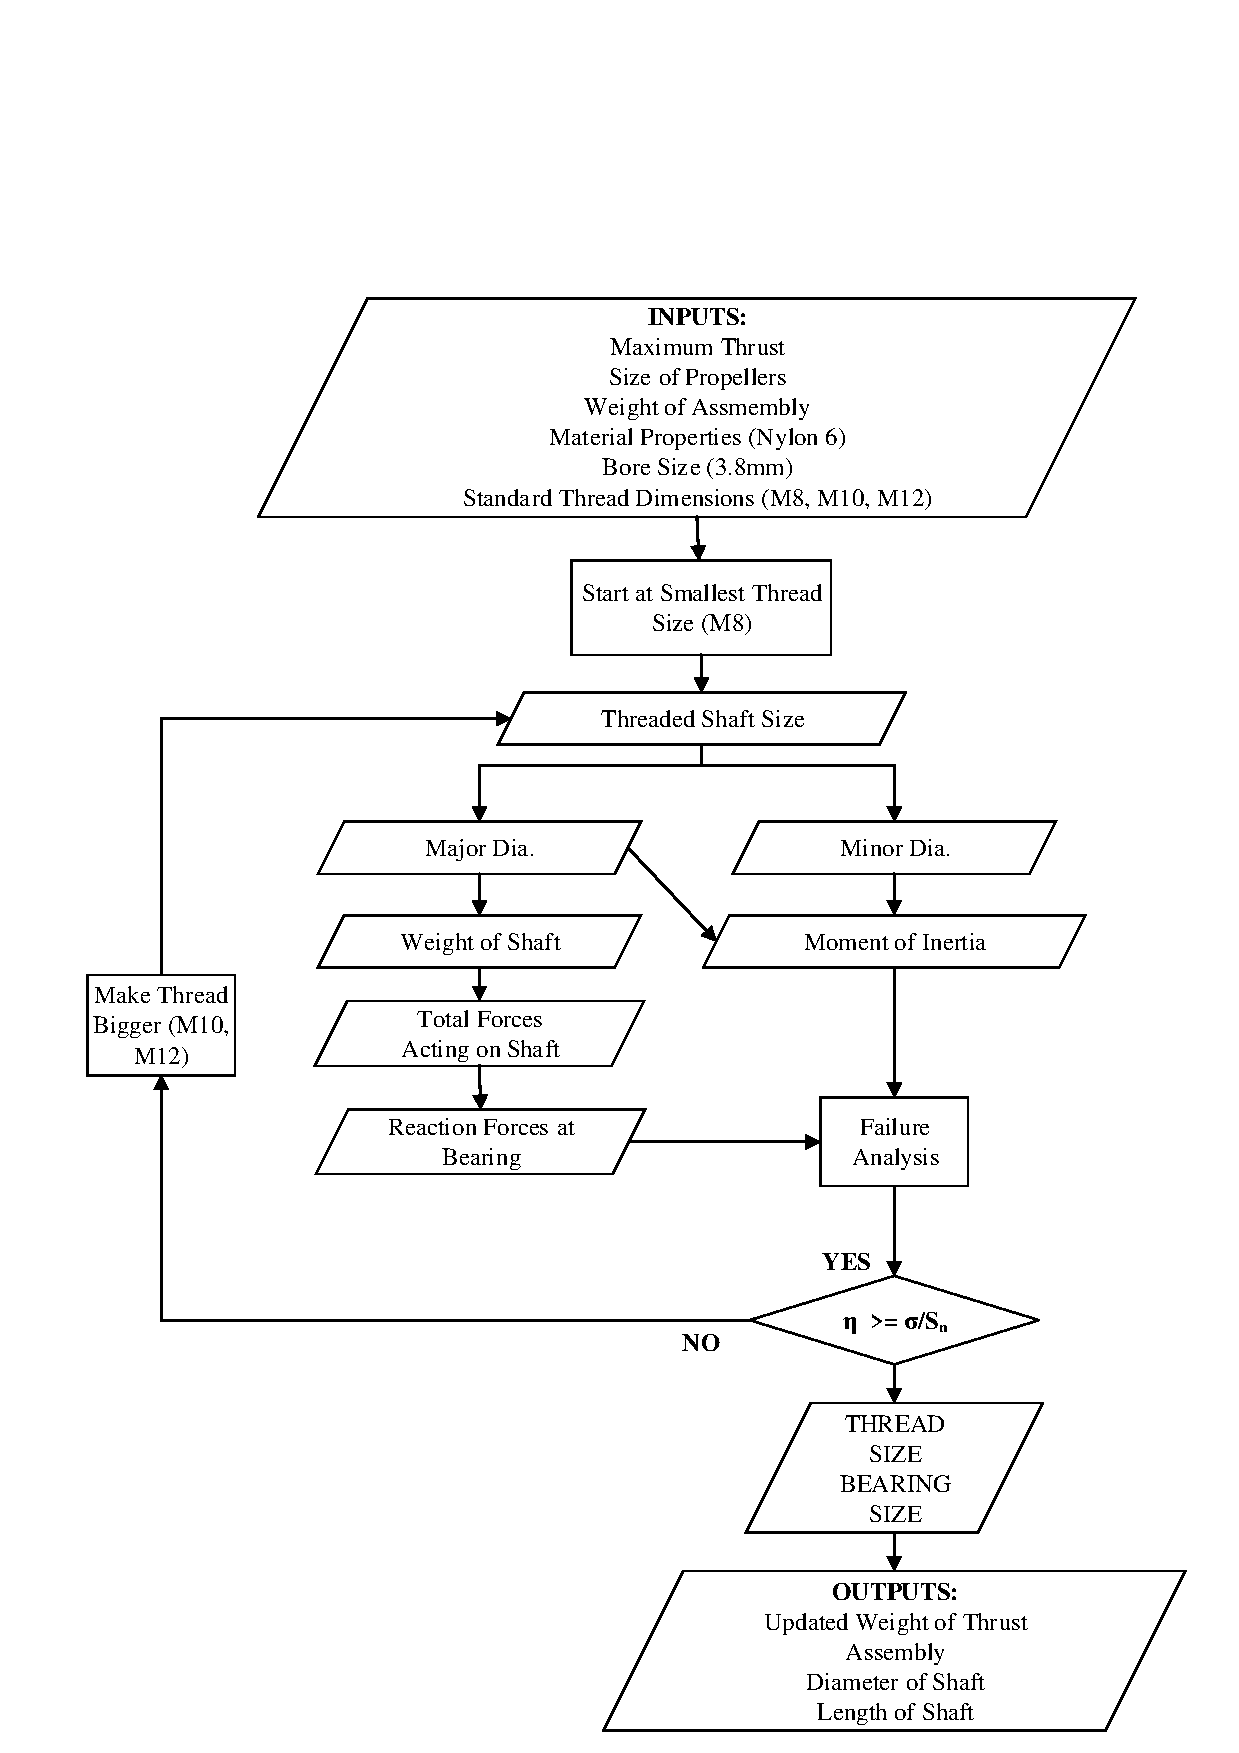
\includegraphics[width=.9\linewidth]{img/paramaterization/thrusterShaft.pdf}
	\caption{Parametrization Outline for the Thruster Shaft}
	\label{fig:ThrusterShaftParametrization}
\end{figure}

The thruster shaft analysis will optimize the diameter of the thruster shaft based on standard threaded shaft dimensions The Analysis will output the diameter of the shaft, the thread of the shaft, the length of the shaft, the weight of the shaft from which it updates the weight and centre of gravity of the entire thruster assembly. The inputs required for the analysis are the maximum thrust, the size of propellers, the weight of the assmembly, the material properties of Nylon 6 REF?? (the shaft material), the bore size of the shaft which is 3.8[mm] and the standard thread dimensions from M8 to M16 REF ??.\\

The material nylon 6 was chosen because of its suitable strength and ease of manufacturability. Aluminium was also considered but would have resulted in an over engineered component or an unproportionally small radius Results that justify this are shown at the end of the section REF??. The bore diameter of 3.8[mm] is based on the screw that attaches the shaft axially to the thrust vectoring motor, shown in FIG ??.\\

The shaft is analysed in simple bending where it is cantilevered at the bearing in the thrust vector motor assembly shown in figure ???. The analysis begins by calculating the required length of shaft for the propeller size and the length 

\end{document}